%!TEX root=../GaugeCNNTheory.tex

\begin{minipage}[t]{\textwidth}
\begin{abstract}

    Motivated by the vast success of deep convolutional networks, there is a great interest in generalizing convolutions to non-Euclidean manifolds.
    A major complication in comparison to flat spaces is that it is unclear in which alignment a convolution kernel should be applied on a manifold.
    The underlying reason for this ambiguity is that general manifolds do not come with a canonical choice of reference frames (gauge).
    Kernels and features therefore have to be expressed relative to \emph{arbitrary coordinates}.
    We argue that the particular choice of coordinatization should not affect a network's inference -- it should be \emph{coordinate independent}.
    A simultaneous demand for coordinate independence and weight sharing is shown to result in a requirement on the network to be \emph{equivariant under local gauge transformations} (changes of local reference frames).
    The ambiguity of reference frames depends thereby on the $G$-\emph{structure} of the manifold,
    such that the necessary level of gauge equivariance is prescribed by the corresponding \emph{structure group}~$G$.
    Coordinate independent convolutions are proven to be equivariant w.r.t. those \emph{isometries} that are symmetries of the $G$-structure.
    The resulting theory is formulated in a coordinate free fashion in terms of fiber bundles.
    To exemplify the design of coordinate independent convolutions, we implement a convolutional network on the M\"obius strip.
    The generality of our differential geometric formulation of convolutional networks is demonstrated by an extensive literature review
    which explains a large number of Euclidean CNNs, spherical CNNs and CNNs on general surfaces as specific instances of coordinate independent convolutions.


    \begin{figure}[H]
        \centering
        \vspace*{2.5ex}
        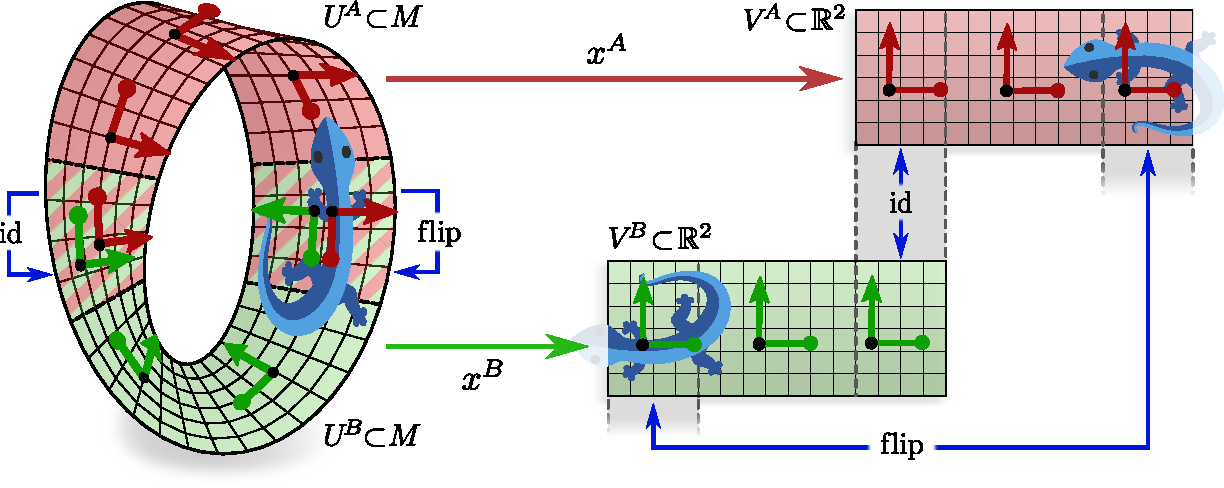
\includegraphics[width=.94\columnwidth]{figures/mobius_conv_gauges.pdf}
    \end{figure}

\end{abstract}

% hack to keep abstract on front page, even though it overflows
\vspace*{-20ex}

\end{minipage}
